\documentclass[12pt,a4paper]{article}
\usepackage{amsmath,amsthm,amssymb,mathtools}
\usepackage{tikz}
\usetikzlibrary{arrows.meta,positioning,shapes.geometric,calc,fit,backgrounds}
\usepackage{graphicx}
\usepackage{booktabs,tabularx,multirow}
\usepackage[ruled,vlined,linesnumbered]{algorithm2e}
\usepackage[most]{tcolorbox}
\usepackage{hyperref}
\usepackage[capitalize,noabbrev]{cleveref}
\usepackage[margin=1in]{geometry}
\usepackage{fancyhdr}
\usepackage{enumitem}
\usepackage{xcolor}

%% ── tcolorbox environments ──────────────────────────────────────────────────
\newtcolorbox{keyinsight}[1][]{colback=blue!5!white,colframe=blue!75!black,fonttitle=\bfseries,title=Key Insight,#1}
\newtcolorbox{example}[1][]{colback=green!5!white,colframe=green!75!black,fonttitle=\bfseries,title=Example,#1}
\newtcolorbox{warningbox}[1][]{colback=red!5!white,colframe=red!75!black,fonttitle=\bfseries,title=Warning,#1}

%% ── amsthm environments ─────────────────────────────────────────────────────
\newtheorem{theorem}{Theorem}[section]
\newtheorem{lemma}[theorem]{Lemma}
\newtheorem{definition}{Definition}[section]
\newtheorem{remark}{Remark}[section]

%% ── Header / Footer ─────────────────────────────────────────────────────────
\pagestyle{fancy}
\fancyhf{}
\rhead{Deep Learning -- Session 13}
\lhead{CNN Hands-on: Convolution, Pooling \& Feature Maps}
\cfoot{\thepage}

%% ── Hyperref setup ───────────────────────────────────────────────────────────
\hypersetup{
  colorlinks=true,
  linkcolor=blue!60!black,
  urlcolor=blue!60!black,
  citecolor=green!50!black
}

%% ── Convenience macros ───────────────────────────────────────────────────────
\newcommand{\relu}{\mathrm{ReLU}}
\newcommand{\stride}{\mathrm{stride}}

% ─────────────────────────────────────────────────────────────────────────────
\begin{document}

% ══════════════════════════════════════════════════════════════════════════════
%  TITLE PAGE
% ══════════════════════════════════════════════════════════════════════════════
\begin{titlepage}
  \centering
  \vspace*{2cm}
  {\LARGE\bfseries Deep Learning\\[0.4em]
   \large IIIT Dharwad -- Online Lecture Series\par}
  \vspace{1.5cm}
  \rule{\textwidth}{1.5pt}\\[0.4em]
  {\Huge\bfseries Session 13\\[0.5em]
   \Large CNN Hands-on:\\[0.3em]
   Convolution, Pooling, and Feature Maps}\\[0.4em]
  \rule{\textwidth}{1.5pt}
  \vspace{1.5cm}

  \begin{tabular}{rl}
    \textbf{Session Number:} & 13 \\[0.3em]
    \textbf{Topic:}          & CNN Hands-on -- Convolution as a Neuron, \\
                             & Output Size Formula, Spatial Dimensions, \\
                             & CNN vs.\ FFNN Comparison \\[0.3em]
    \textbf{Instructors:}    & Prof.\ S R M Prasanna \&\ Dr.\ Sunil Saumya \\[0.3em]
    \textbf{Slides (Deck):}  & \texttt{03-DL-CNN} / \texttt{04-DL-CNN} (Google Colab) \\[0.3em]
    \textbf{Video:}          & \url{https://vimeo.com/1151039438} \\[0.3em]
    \textbf{Duration:}       & $\approx$ 1\,h\,38\,min \\[0.3em]
    \textbf{Date:}           & 2026-03-02 \\
  \end{tabular}

  \vfill
  {\small These notes were compiled from the video lecture transcript and\\
  visual extractions captured from the Vimeo recording.}
\end{titlepage}

% ══════════════════════════════════════════════════════════════════════════════
\tableofcontents
\newpage

% ══════════════════════════════════════════════════════════════════════════════
\section{Introduction}
\label{sec:introduction}
% ══════════════════════════════════════════════════════════════════════════════

Session~13 is a hands-on implementation session for Convolutional Neural
Networks (CNNs).  Building directly on the theoretical overview presented in
Session~12, this session bridges slides and live code in Google Colab,
walking students through

\begin{enumerate}[label=\arabic*.]
  \item the neuronal interpretation of a convolution filter,
  \item the three-stage structure of every CNN layer
        (convolution $\to$ non-linearity $\to$ pooling),
  \item the output-size formula and the conditions under which a given
        combination of input size, filter size, and stride is valid,
  \item a concrete PyTorch implementation of a two-layer CNN applied to the
        Fashion-MNIST dataset, and
  \item a comparative results table showing that a CNN achieves higher
        accuracy and better generalisation with roughly $12\times$ fewer
        parameters than the equivalent Feedforward Neural Network (FFNN).
\end{enumerate}

The session is taught by Dr.\ Sunil Saumya, who leads the students from first
principles through to running, evaluated code.  Prof.\ S R M Prasanna
provided the preceding theoretical session (Session~12).

\begin{keyinsight}
A convolution filter \emph{is} a neuron applied locally: it computes
$\mathbf{w}\cdot\mathbf{x}+b$ over a small spatial patch and then passes the
result through a non-linear activation function.  The crucial additional
property is \textbf{weight sharing} -- the same filter weights are reused at
every spatial position.
\end{keyinsight}

% ══════════════════════════════════════════════════════════════════════════════
\section{Background and Prerequisites}
\label{sec:background}
% ══════════════════════════════════════════════════════════════════════════════

\subsection{Recap of Session 12 (FFNN with Regularisation)}
\label{subsec:recap}

In Session~12 the class built a standard feedforward neural network (FFNN)
trained on the Fashion-MNIST dataset.  The network suffered from
\emph{overfitting}: training accuracy reached $98\,\%$ while evaluation
accuracy stagnated at $88\,\%$.  Three regularisation techniques were
introduced to close this gap:

\begin{itemize}[leftmargin=2em]
  \item \textbf{Dropout:} randomly zeroes activations during training.
  \item \textbf{Batch Normalisation:} normalises intermediate activations to
        stabilise and accelerate training.
  \item \textbf{Weight Decay (L2 regularisation):} penalises large weights in
        the optimiser's update rule.
\end{itemize}

After applying all three techniques the training accuracy dropped to $93\,\%$
while evaluation accuracy held at $88\,\%$, reducing the variance gap from
$10$ to $5$ percentage points.

\subsection{The Neuron Model}
\label{subsec:neuron}

A single neuron performs two operations:
\begin{equation}
  z = \mathbf{w}^{\top}\mathbf{x} + b, \qquad
  a = f(z),
  \label{eq:neuron}
\end{equation}
where $\mathbf{w}$ is the weight vector, $b$ is a scalar bias, $\mathbf{x}$
is the input vector, and $f$ is a non-linear activation function (typically
ReLU in modern networks).  The FFNN uses one weight vector per neuron, and
each neuron is connected to the \emph{entire} input.

\subsection{Why FFNN Falls Short for Images}
\label{subsec:ffnn_limit}

When images are fed to a FFNN, they must first be \emph{flattened} into a
one-dimensional vector.  A $28\times28$ grayscale image becomes a vector of
$784$ elements.  This destroys all spatial structure: the network cannot
exploit the fact that nearby pixels are correlated.  Moreover, the FFNN is
sensitive to translation -- if an object shifts by a few pixels the
representation changes completely, leading to degraded generalisation on
translated test images.

\begin{keyinsight}
CNNs address both shortcomings by (i)~processing the image in 2-D so that
spatial relationships are preserved, and (ii)~using pooling layers to provide
\textbf{translation invariance}.
\end{keyinsight}

% ══════════════════════════════════════════════════════════════════════════════
\section{Convolution as a Neuron with a Local Receptive Field}
\label{sec:conv_neuron}
% ══════════════════════════════════════════════════════════════════════════════

\subsection{Motivation}
\label{subsec:conv_motivation}

The central conceptual move of the session is to reinterpret the convolution
operation as a neuron acting on a \emph{local receptive field}.  In a FFNN,
each neuron sees the whole input.  A convolutional filter neuron sees only a
small patch of size $F\times F$ pixels -- its \emph{receptive field} -- and
the same filter is slid across the entire image.

\subsection{The Convolution Operation}
\label{subsec:conv_op}

Given an input feature map $\mathbf{X}$ of spatial size $N\times N$ and
$C_{\text{in}}$ channels, and a filter (kernel) $\mathbf{W}$ of size
$F\times F\times C_{\text{in}}$, the output at position $(i,j)$ is

\begin{equation}
  z_{i,j} = \sum_{c=1}^{C_{\text{in}}}
             \sum_{p=0}^{F-1}\sum_{q=0}^{F-1}
             W_{p,q,c}\cdot X_{i+p,\,j+q,\,c} + b,
  \label{eq:conv_full}
\end{equation}
followed by the activation
\begin{equation}
  a_{i,j} = f(z_{i,j}).
  \label{eq:conv_act}
\end{equation}

This is identical in form to \cref{eq:neuron} with
$\mathbf{w} \leftrightarrow \mathbf{W}$ (flattened) and
$\mathbf{x} \leftrightarrow$ the local patch.  The output $a_{i,j}$ is one
element of the resulting \textbf{feature map} (also called \emph{activation
map}).

\subsection{Weight Sharing}
\label{subsec:weight_sharing}

A key property that distinguishes convolutional layers from fully connected
layers is \textbf{weight sharing}: the same filter weights $\mathbf{W}$ are
reused at every spatial position $(i,j)$.  This has two major benefits:

\begin{itemize}[leftmargin=2em]
  \item \textbf{Parameter efficiency:} a single $F\times F$ filter has only
        $F^2 C_{\text{in}}$ learnable parameters, regardless of the input
        image size $N$.
  \item \textbf{Equivariance to translation:} if a feature (e.g.\ an edge)
        shifts spatially, the filter produces the same response value at the
        new location.
\end{itemize}

\begin{keyinsight}[title=Key Insight: Weight Sharing]
In a FFNN with input size $N^2$, one hidden neuron has $N^2$ independent
weights.  A convolutional filter with kernel size $F^2$ has only $F^2$
weights regardless of $N$ -- and those weights are shared across all $N^2$
positions.  This is the primary source of CNN's dramatic parameter reduction.
\end{keyinsight}

\subsection{TikZ Diagram: Convolution as a Neuron}
\label{subsec:conv_diagram}

\Cref{fig:conv_neuron} illustrates the local receptive field concept.

\begin{figure}[ht]
\centering
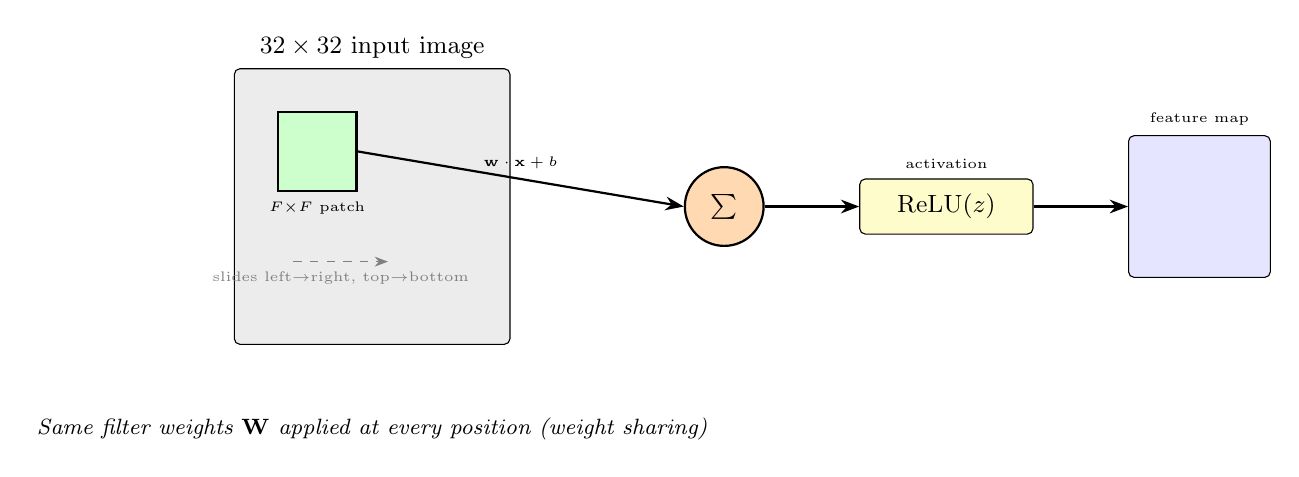
\begin{tikzpicture}[
  >=Stealth,
  every node/.style={font=\small},
  box/.style={draw, minimum width=1.2cm, minimum height=1.2cm,
              fill=gray!15, rounded corners=2pt},
  patch/.style={draw, thick, minimum width=1.0cm, minimum height=1.0cm,
                fill=green!20},
  neuron/.style={draw, circle, minimum size=1.0cm,
                 fill=orange!30, thick},
  outbox/.style={draw, minimum width=2.2cm, minimum height=0.7cm,
                 fill=yellow!20, rounded corners=2pt}
]
%% input image
\node[box, minimum width=3.5cm, minimum height=3.5cm,
      label=above:{$32\times32$ input image}] (img) at (0,0) {};
%% patch highlight
\node[patch] (patch) at (-0.7,0.7) {};
\node[font=\tiny, below=0pt of patch] {$F{\times}F$ patch};
%% arrow from patch to neuron
\node[neuron, right=2.2cm of img] (neur) {$\sum$};
\draw[->, thick] (patch.east) -- node[above, font=\tiny]{$\mathbf{w}\cdot\mathbf{x}+b$} (neur.west);
%% activation
\node[outbox, right=1.2cm of neur, label=above:{\tiny activation}] (act) {$\relu(z)$};
\draw[->, thick] (neur) -- (act);
%% feature map
\node[box, minimum width=1.8cm, minimum height=1.8cm,
      right=1.2cm of act, fill=blue!10,
      label=above:{\tiny feature map}] (fm) {};
\draw[->, thick] (act) -- (fm);
%% sliding arrow
\draw[->, dashed, gray] (-1.0,-0.7) -- node[below, font=\tiny]{slides left$\to$right, top$\to$bottom} (0.2,-0.7);
%% label
\node[below=0.8cm of img, font=\footnotesize\itshape]
  {Same filter weights $\mathbf{W}$ applied at every position (weight sharing)};
\end{tikzpicture}
\caption{Convolution as a neuron with a local receptive field.
         The filter $\mathbf{W}$ (size $F\times F$) slides across the input
         image, computing a dot product at each position to produce one element
         of the output feature map.  ReLU is applied after each dot product.}
\label{fig:conv_neuron}
\end{figure}

\subsection{Multiple Filters and Multiple Feature Maps}
\label{subsec:multi_filter}

A single convolutional layer typically applies $K$ independent filters
$\mathbf{W}^{(1)}, \ldots, \mathbf{W}^{(K)}$ to the same input.  Each filter
produces one feature map, so the layer output is a 3-D tensor of shape
$(K, N_{\text{out}}, N_{\text{out}})$.  The number of feature maps equals the
number of filters:

\begin{equation}
  \text{number of output feature maps} = K.
  \label{eq:num_fm}
\end{equation}

A common design principle is to \emph{increase} $K$ with depth, compensating
for the spatial shrinkage caused by successive convolution and pooling
operations.

% ══════════════════════════════════════════════════════════════════════════════
\section{Block Diagram of the CNN Architecture}
\label{sec:block_diagram}
% ══════════════════════════════════════════════════════════════════════════════

\subsection{Overall Pipeline}
\label{subsec:overall_pipeline}

A canonical CNN for image classification consists of two sequential modules:

\begin{enumerate}[label=\arabic*.]
  \item \textbf{Feature extractor:} one or more repetitions of
        $(\text{Conv} + \relu) \to \text{Pooling}$.
  \item \textbf{Classifier:} Flatten $\to$ one or more fully connected layers
        $\to$ Softmax output.
\end{enumerate}

Each CNN ``layer'' is itself a three-stage block:

\begin{description}[leftmargin=3em, style=nextline]
  \item[Stage 1 -- Convolution] The filter slides over the input performing
        element-wise multiplication and summation, producing an activation
        map.
  \item[Stage 2 -- Non-linearity] ReLU is applied element-wise:
        $\relu(x) = \max(0, x)$.  This zeroes negative activations and
        introduces the non-linearity required for the network to learn complex
        functions.
  \item[Stage 3 -- Pooling] A pooling window (typically $2\times2$) slides
        over the feature map and retains only the most salient value (max
        pooling) or an aggregate (average pooling), reducing spatial
        dimensions and providing translation invariance.
\end{description}

\subsection{TikZ Diagram: CNN Block Diagram}
\label{subsec:block_tikz}

\Cref{fig:cnn_block} shows the full CNN pipeline from input image to softmax
output.

\begin{figure}[ht]
\centering
\resizebox{\textwidth}{!}{%
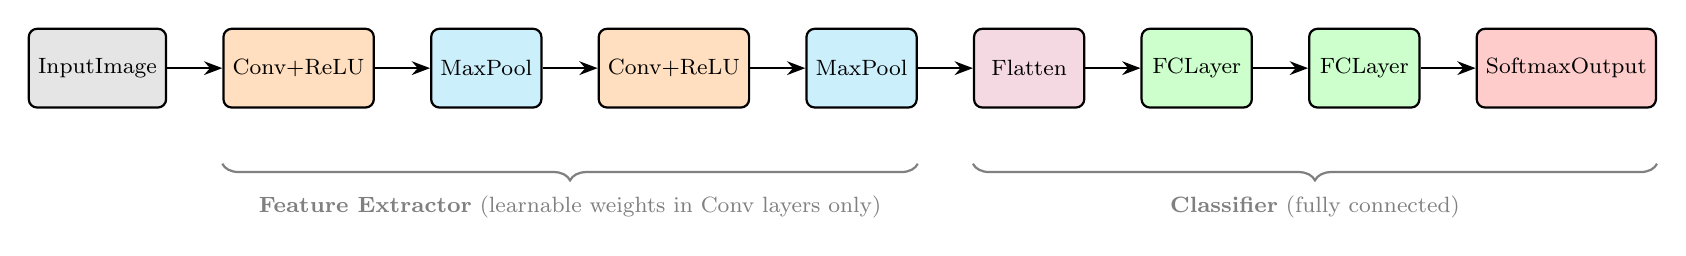
\begin{tikzpicture}[
  >=Stealth,
  every node/.style={font=\footnotesize},
  blk/.style={draw, rounded corners=3pt, minimum width=1.4cm,
              minimum height=1.0cm, text centered, thick},
  arr/.style={->, thick}
]
%% Nodes
\node[blk, fill=gray!20]                               (inp)  {Input\\Image};
\node[blk, fill=orange!25,  right=0.7cm of inp]        (c1)   {Conv\\+ReLU};
\node[blk, fill=cyan!20,    right=0.7cm of c1]         (p1)   {Max\\Pool};
\node[blk, fill=orange!25,  right=0.7cm of p1]         (c2)   {Conv\\+ReLU};
\node[blk, fill=cyan!20,    right=0.7cm of c2]         (p2)   {Max\\Pool};
\node[blk, fill=purple!15,  right=0.7cm of p2]         (fl)   {Flatten};
\node[blk, fill=green!20,   right=0.7cm of fl]         (fc1)  {FC\\Layer};
\node[blk, fill=green!20,   right=0.7cm of fc1]        (fc2)  {FC\\Layer};
\node[blk, fill=red!20,     right=0.7cm of fc2]        (sm)   {Softmax\\Output};

%% Arrows
\draw[arr] (inp) -- (c1);
\draw[arr] (c1)  -- (p1);
\draw[arr] (p1)  -- (c2);
\draw[arr] (c2)  -- (p2);
\draw[arr] (p2)  -- (fl);
\draw[arr] (fl)  -- (fc1);
\draw[arr] (fc1) -- (fc2);
\draw[arr] (fc2) -- (sm);

%% Braces / labels below
\draw[decorate, decoration={brace,amplitude=6pt,mirror},
      thick, gray]
  ([yshift=-0.7cm]c1.south west) -- ([yshift=-0.7cm]p2.south east)
  node[midway, below=8pt] {\textbf{Feature Extractor} (learnable weights in Conv layers only)};

\draw[decorate, decoration={brace,amplitude=6pt,mirror},
      thick, gray]
  ([yshift=-0.7cm]fl.south west) -- ([yshift=-0.7cm]sm.south east)
  node[midway, below=8pt] {\textbf{Classifier} (fully connected)};
\end{tikzpicture}}
\caption{Block diagram of a CNN with two convolution--pooling stages followed
         by fully-connected classification layers.  The pooling layers have no
         learnable weights; only the convolutional and fully-connected layers
         participate in backpropagation.}
\label{fig:cnn_block}
\end{figure}

\subsection{Where Are the Neurons?}
\label{subsec:where_neurons}

A natural question is: where do neurons appear in the CNN pipeline?

\begin{itemize}[leftmargin=2em]
  \item \textbf{Convolution layer:} every output element $a_{i,j}^{(k)}$ is
        produced by a neuron-like operation (weighted sum $+$ bias $+$
        activation).  Weights \emph{are} learned here via backpropagation.
  \item \textbf{Pooling layer:} no weighted sum, no learnable weights.  This
        is a fixed aggregation operation (max / average).  No
        backpropagation through learnable parameters occurs here.
  \item \textbf{Flatten layer:} purely a shape transformation (2-D
        $\to$ 1-D); no learnable parameters.
  \item \textbf{Fully connected layers:} standard neurons, each connected to
        all elements of the preceding feature vector.
\end{itemize}

\begin{remark}
Pooling is an \emph{optional} layer.  Modern architectures (e.g.\
ResNets) sometimes use strided convolutions instead of pooling to reduce
spatial dimensions, or omit pooling entirely in certain stages.
\end{remark}

% ══════════════════════════════════════════════════════════════════════════════
\section{Convolution Output Size Formula}
\label{sec:output_size}
% ══════════════════════════════════════════════════════════════════════════════

\subsection{Derivation}
\label{subsec:derivation}

Consider a 1-D input of length $N$, a filter of size $F$, and a stride of
$S$.  Starting at position $0$, the filter can be placed at positions
$0, S, 2S, \ldots$ as long as the filter does not exceed the input boundary.
The last valid start position is $N - F$, which is reached in
$\lfloor(N-F)/S\rfloor$ steps.  Including the initial position, the total
number of valid placements -- equivalently, the output size -- is

\begin{equation}
  \boxed{N_{\text{out}} = \left\lfloor \frac{N - F}{S} \right\rfloor + 1.}
  \label{eq:output_size}
\end{equation}

For integer outputs this requires $(N - F)$ to be divisible by $S$.  When
this condition is not met, PyTorch raises a runtime error.

\subsection{Effect of Zero-Padding}
\label{subsec:padding}

Zero-padding adds $P$ rows (and columns) of zeros around the input, making
the effective input size $N + 2P$.  \Cref{eq:output_size} becomes

\begin{equation}
  N_{\text{out}} = \left\lfloor \frac{N + 2P - F}{S} \right\rfloor + 1.
  \label{eq:output_size_pad}
\end{equation}

Setting $P = (F-1)/2$ (``same'' padding, valid for odd $F$ with $S=1$)
ensures $N_{\text{out}} = N$, i.e.\ the feature map has the same spatial
dimensions as the input.

\begin{definition}[Valid Convolution Configuration]
\label{def:valid_config}
A combination $(N, F, S)$ is \emph{valid} if and only if $(N - F)$ is
exactly divisible by $S$, i.e.\ $(N - F) \bmod S = 0$.
\end{definition}

\subsection{Worked Examples (from the Lecture)}
\label{subsec:worked_examples}

The instructor worked through the following three cases using a
$7\times7$ input and a $3\times3$ filter:

\begin{table}[ht]
\centering
\caption{Output size for a $7\times7$ input with $3\times3$ filter at varying
         strides. Only integer outputs are valid.}
\label{tab:stride_examples}
\begin{tabular}{cccc}
\toprule
\textbf{Input ($N$)} & \textbf{Filter ($F$)} & \textbf{Stride ($S$)} &
\textbf{Output size} \\
\midrule
7 & 3 & 1 & $(7-3)/1 + 1 = \mathbf{5}$ \quad (valid) \\
7 & 3 & 2 & $(7-3)/2 + 1 = \mathbf{3}$ \quad (valid) \\
7 & 3 & 3 & $(7-3)/3 + 1 = 2.33\ldots$ \quad \textbf{invalid} \\
\bottomrule
\end{tabular}
\end{table}

\begin{warningbox}
If $(N-F)/S$ is not an integer, the convolution is \textbf{invalid}.  PyTorch
will raise a \texttt{RuntimeError} and refuse to run the forward pass.
Never assume that any combination of input size, filter size, and stride will
work -- always verify with \cref{eq:output_size} before building the model.
\end{warningbox}

\subsection{Applying the Formula: $32\times32$ Input with $5\times5$ Filter}
\label{subsec:formula_32}

The lecture uses this example to explain why the first feature map in the
canonical CNN diagram has spatial size $28\times28$:

\begin{align}
  N &= 32, \quad F = 5, \quad S = 1, \quad P = 0 \notag \\
  N_{\text{out}} &= \frac{32 - 5}{1} + 1 = 28.
  \label{eq:32to28}
\end{align}

\begin{example}
\textbf{Verifying the $7\times7 \to 5\times5$ case.}

Input: $7\times7$; filter: $3\times3$; stride: $1$.
\[
  N_{\text{out}} = \frac{7 - 3}{1} + 1 = 5.
\]
The filter can scan 5 positions left-to-right and 5 positions top-to-bottom,
producing a $5\times5$ output matrix with exactly 25 scalar values.
\end{example}

% ══════════════════════════════════════════════════════════════════════════════
\section{Pooling Operations}
\label{sec:pooling}
% ══════════════════════════════════════════════════════════════════════════════

\subsection{Max Pooling}
\label{subsec:max_pool}

Max pooling slides a window of size $P_w \times P_w$ over the feature map
with stride $S_p$ and retains the maximum value in each window:

\begin{equation}
  y_{i,j} = \max_{0 \le p < P_w,\; 0 \le q < P_w}
             a_{iS_p + p,\; jS_p + q}.
  \label{eq:maxpool}
\end{equation}

A $2\times2$ window with stride $2$ halves both spatial dimensions, so a
$28\times28$ feature map becomes $14\times14$.

\subsection{Average Pooling}
\label{subsec:avg_pool}

Average pooling replaces the $\max$ in \cref{eq:maxpool} with the arithmetic
mean:
\begin{equation}
  y_{i,j} = \frac{1}{P_w^2}
             \sum_{p=0}^{P_w-1}\sum_{q=0}^{P_w-1}
             a_{iS_p + p,\; jS_p + q}.
  \label{eq:avgpool}
\end{equation}

\subsection{Why Pooling Provides Translation Invariance}
\label{subsec:pool_invariance}

If a feature (e.g.\ a detected edge) shifts by one pixel, the max-pooling
window may still capture the same maximum value.  Repeated pooling layers
accumulate this robustness, so that the final feature vector is approximately
invariant to small spatial translations of the input.

\begin{keyinsight}[title=Key Insight: Translation Invariance]
Max pooling retains the strongest activation within each local window,
regardless of its precise position.  After two pooling layers, the CNN
``knows'' that a feature is present in a neighbourhood, not at a specific
pixel.  This is why CNNs generalise better to translated images than FFNNs
(see \cref{tab:cnn_vs_ffnn}).
\end{keyinsight}

\subsection{Pooling Output Size}
\label{subsec:pool_size}

The output size formula for pooling is the same as for convolution,
\cref{eq:output_size}, with $N \leftarrow N_{\text{feature map}}$,
$F \leftarrow P_w$, and $S \leftarrow S_p$.  With $P_w = 2$ and $S_p = 2$:

\begin{equation}
  N_{\text{pool}} = \frac{N_{\text{feature map}} - 2}{2} + 1
                  = \frac{N_{\text{feature map}}}{2}.
  \label{eq:pool_size}
\end{equation}

\subsection{Comparing Convolution and Pooling Layers}

\begin{table}[ht]
\centering
\caption{Comparison of convolutional and pooling layers.}
\label{tab:conv_vs_pool}
\begin{tabular}{lcc}
\toprule
\textbf{Property} & \textbf{Convolution Layer} & \textbf{Pooling Layer} \\
\midrule
Operation & Weighted sum $+$ bias & Max / average \\
Learnable weights & Yes & No \\
Activation function & Yes (ReLU) & No \\
Spatial size change & Reduces by $(F-1)/S$ & Reduces by factor $S_p$ \\
Feature channels & Increases (more filters) & Unchanged \\
Participates in backprop & Yes & No (fixed) \\
Optional in CNN & No (core layer) & Yes (can be skipped) \\
\bottomrule
\end{tabular}
\end{table}

% ══════════════════════════════════════════════════════════════════════════════
\section{Hierarchical Feature Learning}
\label{sec:hierarchical}
% ══════════════════════════════════════════════════════════════════════════════

A deep CNN extracts features at increasing levels of abstraction:

\begin{enumerate}[label=\textbf{Layer \arabic*:}]
  \item \textbf{Low-level features} -- horizontal edges, vertical edges,
        diagonal edges, colour blobs.  These are detected by the first
        convolution layer's filters, whose receptive field is small (e.g.\
        $3\times3$).
  \item \textbf{Mid-level features} -- combinations of edges forming corners,
        textures, simple shapes.  The second convolution layer's filters see
        the output of the first pooling layer and can combine primitives over
        a larger effective receptive field.
  \item \textbf{High-level features} -- object parts (e.g.\ wheel shape, eye
        pattern, fur texture).  Deeper layers accumulate evidence from wider
        input regions.
  \item \textbf{Classification} -- the fully connected head receives a
        flattened high-level feature vector and maps it to class logits via
        learned linear transformations, with a softmax at the output.
\end{enumerate}

\begin{remark}
The filter weights that produce these hierarchical features are never
manually designed.  They are initialised randomly and learnt entirely through
backpropagation on labelled training data.  The ``edge detectors'' in early
layers emerge automatically as the most useful low-level basis for the task.
\end{remark}

% ══════════════════════════════════════════════════════════════════════════════
\section{Spatial Dimensions: A Closer Look}
\label{sec:spatial}
% ══════════════════════════════════════════════════════════════════════════════

\subsection{Stride and Feature Resolution}
\label{subsec:stride_resolution}

Stride controls the resolution of the output feature map:

\begin{itemize}[leftmargin=2em]
  \item \textbf{Stride $= 1$:} the filter visits every pixel.  All fine-grained
        spatial detail is captured.  Preferred when every local feature is
        important.
  \item \textbf{Stride $= 2$:} the filter skips alternate positions.  Spatial
        resolution is halved.  Some fine detail is lost, but computation is
        reduced by $4\times$ (fewer output elements).
  \item \textbf{Stride $> 2$:} increasingly coarse feature maps.  Used in
        the first layer of large-scale models (e.g.\ AlexNet uses stride 4
        on the first $11\times11$ layer) to rapidly reduce the spatial footprint
        of a high-resolution input.
\end{itemize}

\begin{example}
\textbf{Effect of stride on a $7\times7$ input with $3\times3$ filter.}
\begin{align*}
  S=1: &\quad N_{\text{out}} = (7-3)/1 + 1 = 5. \quad \text{fine-grained} \\
  S=2: &\quad N_{\text{out}} = (7-3)/2 + 1 = 3. \quad \text{coarser} \\
  S=3: &\quad N_{\text{out}} = (7-3)/3 + 1 = 2.33\ldots \quad
              \text{\textbf{invalid}} \\
\end{align*}
With stride~3, the filter cannot tile the $7\times7$ grid cleanly.  After the
second placement the filter would require a third column that does not exist
(only 1 column remains, but 3 are needed for the filter).
\end{example}

\subsection{Design Rule for Valid Configurations}
\label{subsec:valid_rule}

\begin{theorem}[Valid Stride Condition]
\label{thm:valid_stride}
A convolution on a spatial dimension of size $N$ with filter size $F$ and
stride $S$ (and no padding) is valid if and only if
\begin{equation}
  (N - F) \bmod S = 0.
  \label{eq:valid_cond}
\end{equation}
\end{theorem}

\begin{proof}
The filter must reach position $N-F$ (the last valid starting position) in an
integer number of stride steps from position $0$.  This requires
$(N-F) / S \in \mathbb{Z}_{\geq 0}$, i.e.\ $(N-F)$ divisible by $S$.
\end{proof}

% ══════════════════════════════════════════════════════════════════════════════
\section{PyTorch Implementation of a Two-Layer CNN}
\label{sec:pytorch}
% ══════════════════════════════════════════════════════════════════════════════

\subsection{Dataset: Fashion-MNIST}
\label{subsec:dataset}

The session uses the Fashion-MNIST dataset (\texttt{04-DL-CNN} Colab notebook):
\begin{itemize}[leftmargin=2em]
  \item 60\,000 training images $+$ 10\,000 test images.
  \item Each image: $28\times28$ grayscale pixels, 10 classes
        (T-shirt, trouser, pullover, dress, coat, sandal, shirt, sneaker,
        bag, ankle boot).
  \item Original CSV format: each row is one flattened image (784 pixel
        values) with a label in the first column.
\end{itemize}

For the CNN, the 784-element rows are \textbf{reshaped} to
$(1, 28, 28)$ tensors (batch dimension is handled by the DataLoader):
\begin{equation}
  \text{shape} = (\text{batch\_size},\; C_{\text{in}},\; H,\; W)
               = (\text{-}1,\; 1,\; 28,\; 28).
  \label{eq:data_shape}
\end{equation}

\subsection{Network Architecture}
\label{subsec:architecture}

The CNN defined in the notebook has the following structure:

\paragraph{Feature Extractor (Sequential container 1)}
\begin{enumerate}[label=\textbf{\arabic*.}]
  \item \texttt{Conv2d}(in\_channels=1, out\_channels=32,
        kernel\_size=3, stride=1, padding=``same'', bias=True)
  \item \texttt{ReLU}
  \item \texttt{BatchNorm2d}(32)
  \item \texttt{MaxPool2d}(kernel\_size=2, stride=2)
        \hfill $28\times28 \to 14\times14$
  \item \texttt{Conv2d}(in\_channels=32, out\_channels=64,
        kernel\_size=3, stride=1, padding=``same'', bias=True)
  \item \texttt{ReLU}
  \item \texttt{BatchNorm2d}(64)
  \item \texttt{MaxPool2d}(kernel\_size=2, stride=2)
        \hfill $14\times14 \to 7\times7$
\end{enumerate}

\paragraph{Classifier (Sequential container 2, after Flatten)}
\begin{enumerate}[label=\textbf{\arabic*.}]
  \item \texttt{Linear}($64\times7\times7 = 3136 \to 128$)
  \item \texttt{ReLU}
  \item \texttt{Linear}($128 \to 64$)
  \item \texttt{ReLU}
  \item \texttt{Linear}($64 \to 10$)
\end{enumerate}

\subsection{Parameter Count Analysis}
\label{subsec:param_count}

\Cref{tab:param_count} summarises the learnable parameters per layer.

\begin{table}[ht]
\centering
\caption{Learnable parameter count for each layer of the CNN.}
\label{tab:param_count}
\begin{tabular}{lrr}
\toprule
\textbf{Layer} & \textbf{Shape} & \textbf{Parameters} \\
\midrule
Conv2d-1 (weights) & $32\times1\times3\times3$ & 288 \\
Conv2d-1 (bias)    & $32$                       & 32  \\
BatchNorm2d-1      & $2\times32$                & 64  \\
Conv2d-2 (weights) & $64\times32\times3\times3$ & 18\,432 \\
Conv2d-2 (bias)    & $64$                       & 64  \\
BatchNorm2d-2      & $2\times64$                & 128 \\
Linear-1           & $3136\times128$            & 401\,408 \\
Linear-1 (bias)    & $128$                      & 128 \\
Linear-2           & $128\times64$              & 8\,192 \\
Linear-2 (bias)    & $64$                       & 64  \\
Linear-3           & $64\times10$               & 640 \\
Linear-3 (bias)    & $10$                       & 10  \\
\midrule
\textbf{Total (approx.)} & & $\sim$\,3\,142 \\
\bottomrule
\end{tabular}
\end{table}

\subsection{Training Algorithm}
\label{subsec:training}

\begin{algorithm}[H]
\caption{Mini-Batch Training of CNN (Fashion-MNIST)}
\label{alg:cnn_train}
\DontPrintSemicolon
\SetAlgoLined
\KwIn{Training set $\mathcal{D}_{\text{train}}$, batch size $B=32$,
      epochs $T$, learning rate $\eta$, weight decay $\lambda$}
\KwOut{Trained CNN parameters $\theta$}

Initialise $\theta$ randomly (Kaiming uniform for Conv/Linear)\;
\For{$t = 1$ \KwTo $T$}{
  \ForEach{mini-batch $(X_b, y_b)$ from $\mathcal{D}_{\text{train}}$}{
    Reshape $X_b$ to shape $(B, 1, 28, 28)$\;
    \tcp{Forward pass}
    $\hat{y}_b \leftarrow \mathrm{CNN}_\theta(X_b)$
    \tcp*{logits, shape $(B, 10)$}
    $\mathcal{L} \leftarrow \mathrm{CrossEntropy}(\hat{y}_b,\, y_b)$\;
    \tcp{Backward pass}
    Zero gradients: $\nabla_\theta \leftarrow \mathbf{0}$\;
    $\nabla_\theta \leftarrow \partial\mathcal{L}/\partial\theta$
    \tcp*{backpropagation}
    \tcp{Parameter update (Adam with weight decay)}
    $\theta \leftarrow \theta - \eta\,\nabla_\theta - \eta\lambda\,\theta$\;
  }
  Evaluate on validation set; log accuracy\;
}
\Return $\theta$\;
\end{algorithm}

% ══════════════════════════════════════════════════════════════════════════════
\section{CNN vs.\ FFNN: Comparative Results}
\label{sec:results}
% ══════════════════════════════════════════════════════════════════════════════

\subsection{Experimental Setup}
\label{subsec:exp_setup}

Both models are trained on the Fashion-MNIST \emph{two-class} subset
(binary classification) to make the comparison controlled.  The same
training procedure (Adam optimiser, same number of epochs, same batch size)
is applied to both models.  Two evaluation conditions are used:

\begin{enumerate}[label=\arabic*.]
  \item \textbf{Original images:} test set without any augmentation.
  \item \textbf{Translated images:} test images shifted by a few pixels,
        simulating a distribution shift that breaks spatial position
        assumptions.
\end{enumerate}

\subsection{Results Table}
\label{subsec:results_table}

\begin{table}[ht]
\centering
\caption{CNN vs.\ FFNN: parameter count and test accuracy on original
         and translated Fashion-MNIST images (two-class subset).}
\label{tab:cnn_vs_ffnn}
\begin{tabular}{lrcc}
\toprule
\multirow{2}{*}{\textbf{Model}} &
\multirow{2}{*}{\textbf{Parameters}} &
\multicolumn{2}{c}{\textbf{Test Accuracy}} \\
\cmidrule(lr){3-4}
 & & \textbf{Original} & \textbf{Translated} \\
\midrule
FFNN  & 39\,352 & 96.47\,\%  & 80.42\,\% \\
CNN   & 3\,142  & $\approx$98\,\%  & 88.26\,\% \\
\midrule
\textbf{Improvement} & $12\times$ fewer & $+1.5$\,pp & $+7.8$\,pp \\
\bottomrule
\end{tabular}
\end{table}

\subsection{Analysis of Results}
\label{subsec:analysis}

\Cref{tab:cnn_vs_ffnn} reveals three important findings:

\begin{enumerate}[label=\arabic*.]
  \item \textbf{Parameter efficiency.}  The CNN achieves better accuracy
        with $12\times$ fewer parameters ($3\,142$ vs.\ $39\,352$).  This
        results directly from weight sharing in convolutional layers: a
        $3\times3$ filter has only 9 weights regardless of input size.
  \item \textbf{Higher accuracy on original images.}  CNN reaches
        $\approx 98\,\%$ vs.\ FFNN's $96.47\,\%$.  Exploiting spatial
        structure leads to better feature representations.
  \item \textbf{Dramatically better generalisation to translated images.}
        CNN achieves $88.26\,\%$ vs.\ FFNN's $80.42\,\%$ on translated
        inputs -- a gap of $7.8$ percentage points.  This confirms the
        translation invariance benefit of max-pooling layers.
\end{enumerate}

\begin{keyinsight}[title=Key Insight: Why CNN Handles Translation]
FFNN memorises the exact pixel positions of features.  When an image is
shifted, the pixel values appear at new indices and the FFNN ``sees'' an
unfamiliar pattern.  The CNN's pooling layers aggregate over small
neighbourhoods, making the representation robust to small shifts.
\end{keyinsight}

% ══════════════════════════════════════════════════════════════════════════════
\section{Live Visualisation: Convolution and Pooling in Action}
\label{sec:visualisation}
% ══════════════════════════════════════════════════════════════════════════════

During the session the instructor demonstrated convolution using the
\texttt{deeplizard} interactive visualisation website with Fashion-MNIST
images.  Key observations:

\begin{enumerate}[label=\arabic*.]
  \item \textbf{Filter sliding:} the $3\times3$ window moves left-to-right,
        top-to-bottom across the image with stride~1.  At each position, nine
        element-wise multiplications are summed to give one output scalar.
  \item \textbf{Edge detection:} a ``top-edge'' filter (weights structured to
        respond to horizontal transitions) produces high (positive, red)
        activations at top edges and low (negative, blue) activations
        elsewhere.
  \item \textbf{ReLU effect:} all negative (blue) values are zeroed by ReLU,
        leaving only the detected edge features.
  \item \textbf{Filter direction:} swapping to a ``right-edge'' filter
        shifts the strong activations to the right side of the image,
        confirming that filter weights determine what feature is extracted.
  \item \textbf{Learnt filters:} in a real CNN, filter weights are not
        hand-designed.  They are initialised randomly and optimised via
        backpropagation; the network learns which features are useful for
        the task.
  \item \textbf{Max pooling:} the pooling demo showed a $2\times2$ window
        with stride~2.  Each window retains its maximum; a $4\times4$ feature
        map is reduced to $2\times2$.
\end{enumerate}

% ══════════════════════════════════════════════════════════════════════════════
\section{Design Choices and Hyperparameters}
\label{sec:design}
% ══════════════════════════════════════════════════════════════════════════════

\subsection{Choosing the Number of Filters}
\label{subsec:num_filters}

Selecting the number of filters per layer is more art than science:

\begin{itemize}[leftmargin=2em]
  \item There is no analytic formula for the optimal number of filters.
  \item A common heuristic: \emph{increase} the number of filters as depth
        increases, to compensate for the shrinking spatial dimensions and
        prevent information bottlenecks.  The lecture example uses 32 filters
        in layer~1 and 64 in layer~2.
  \item The practical approach is to start with a reasonable number and tune
        by observing validation accuracy.
\end{itemize}

\subsection{Kernel / Filter Terminology}
\label{subsec:terminology}

The terms \emph{kernel} and \emph{filter} are often used interchangeably in
the literature.  One useful convention adopted in the lecture:

\begin{itemize}[leftmargin=2em]
  \item \textbf{Kernel:} the weight matrix itself (e.g.\ a $3\times3$ array
        of floats).
  \item \textbf{Filter:} a collection of kernels -- one per input channel --
        that together produce one output feature map.  For a 3-channel (RGB)
        input with a $5\times5$ kernel, each filter contains
        $3 \times 5 \times 5 = 75$ weights.
\end{itemize}

\subsection{Choosing Stride}
\label{subsec:choosing_stride}

\begin{itemize}[leftmargin=2em]
  \item \textbf{Stride 1:} maximum feature resolution.  Recommended when
        the image contains dense information throughout (e.g.\ texture
        classification, medical imaging).
  \item \textbf{Stride 2:} halves the feature map size, reducing memory and
        computation.  Commonly used in pooling layers and sometimes in strided
        convolutions as a pooling substitute.
  \item Always verify that $(N - F) \bmod S = 0$ before training; otherwise
        PyTorch will raise an error.
\end{itemize}

% ══════════════════════════════════════════════════════════════════════════════
\section{Connecting Convolution to the Full CNN Forward Pass}
\label{sec:forward_pass}
% ══════════════════════════════════════════════════════════════════════════════

\subsection{Dimension Trace Through the Network}
\label{subsec:dim_trace}

Starting from a single $28\times28$ grayscale image, the spatial and channel
dimensions evolve as follows through the two-layer CNN:

\begin{align}
  \text{Input:} &\quad (1,\; 28,\; 28) \notag \\
  \text{After Conv2d-1 (same padding):} &\quad (32,\; 28,\; 28) \notag \\
  \text{After MaxPool2d (2, stride=2):} &\quad (32,\; 14,\; 14) \notag \\
  \text{After Conv2d-2 (same padding):} &\quad (64,\; 14,\; 14) \notag \\
  \text{After MaxPool2d (2, stride=2):} &\quad (64,\; 7,\; 7) \notag \\
  \text{After Flatten:} &\quad (3136,) \notag \\
  \text{After Linear-1:} &\quad (128,) \notag \\
  \text{After Linear-2:} &\quad (64,) \notag \\
  \text{After Linear-3 (logits):} &\quad (10,) \notag \\
  \text{After Softmax:} &\quad (10,) \quad \text{probabilities}
  \label{eq:dim_trace}
\end{align}

The flatten step converts the $(64, 7, 7)$ tensor to a $64\times7\times7 =
3136$-dimensional vector before the first linear layer.

\subsection{Cross-Entropy Loss}
\label{subsec:loss}

The network is trained with cross-entropy loss:
\begin{equation}
  \mathcal{L} = -\sum_{c=1}^{C} y_c \log \hat{p}_c,
  \label{eq:crossentropy}
\end{equation}
where $y_c \in \{0,1\}$ is the one-hot true label and $\hat{p}_c$ is the
predicted probability for class $c$.  Backpropagation computes gradients of
$\mathcal{L}$ with respect to all learnable parameters (Conv and Linear
weights and biases; BatchNorm scale and shift), which are then updated by the
Adam optimiser.

% ══════════════════════════════════════════════════════════════════════════════
\section{Summary and Conclusions}
\label{sec:summary}
% ══════════════════════════════════════════════════════════════════════════════

\subsection{Lecture Summary}
\label{subsec:lecture_summary}

Session~13 provided a comprehensive hands-on treatment of Convolutional
Neural Networks, covering:

\begin{enumerate}[label=\arabic*., leftmargin=2.5em]
  \item \textbf{Conceptual foundation:} A convolutional filter is a neuron
        applied locally, performing the same $\mathbf{w}\cdot\mathbf{x}+b$
        computation as any fully connected neuron, but restricted to a small
        receptive field and with weights shared across all spatial positions.
  \item \textbf{CNN architecture:} the three-stage layer structure
        (Conv $\to$ ReLU $\to$ Pooling), the flatten bridge, and the
        fully-connected classifier.
  \item \textbf{Output-size formula:}
        $N_{\text{out}} = \lfloor(N-F)/S\rfloor + 1$, with the validity
        condition $(N-F) \bmod S = 0$ enforced by PyTorch at runtime.
  \item \textbf{Worked examples} for a $7\times7$ input with a $3\times3$
        filter at strides 1, 2, and 3 (the last being invalid).
  \item \textbf{Pooling:} max pooling as a fixed aggregation operation that
        reduces spatial dimensions and introduces translation invariance.
        No learnable weights; optional but strongly recommended.
  \item \textbf{PyTorch implementation:} two convolutional blocks
        ($32$~filters then $64$~filters) followed by a three-layer
        fully-connected classifier, yielding $\sim$3\,142 total parameters.
  \item \textbf{Comparative results:} CNN achieves $\approx98\,\%$ accuracy
        on original images and $88.26\,\%$ on translated images, versus
        $96.47\,\%$ and $80.42\,\%$ for the FFNN -- with $12\times$ fewer
        parameters.
\end{enumerate}

\subsection{Key Takeaways}
\label{subsec:takeaways}

\begin{keyinsight}[title=Key Takeaway 1 -- Parameter Efficiency]
Weight sharing in convolutional layers is the primary mechanism behind CNN's
dramatic parameter reduction.  A $3\times3$ filter has only 9 weights
regardless of input size, compared to $N^2$ weights for a fully connected
neuron on an $N\times N$ image.
\end{keyinsight}

\begin{keyinsight}[title=Key Takeaway 2 -- Translation Invariance]
Max-pooling layers aggregate the strongest activations over local
neighbourhoods, making the feature representation approximately invariant to
small translations.  This is directly reflected in the results: CNN drops only
$\sim$10 pp on translated images versus $\sim$16 pp for FFNN.
\end{keyinsight}

\begin{keyinsight}[title=Key Takeaway 3 -- Validity of Configurations]
Not all combinations of input size, filter size, and stride are valid.  Always
verify $(N-F)\bmod S = 0$ before committing to a network architecture.  Use
``same'' padding when you want the feature map to match the input size.
\end{keyinsight}

\subsection{Looking Ahead}
\label{subsec:ahead}

The session explicitly noted that CNN material will continue for one or two
more sessions, covering:

\begin{itemize}[leftmargin=2em]
  \item Deeper and more complex CNN architectures (beyond two conv layers).
  \item \texttt{Conv1d} for sequential / text data.
  \item Possibly canonical architectures such as LeNet, AlexNet, or VGGNet.
  \item Full 10-class Fashion-MNIST CNN results.
\end{itemize}

\vspace{1.5em}
\noindent\rule{\textwidth}{0.5pt}\\[0.3em]
{\small\itshape
These notes are derived from the recorded lecture available at
\url{https://vimeo.com/1151039438} and the slides at
\url{https://learning.iiitdwd.ac.in/mod/pdfprotect/view.php?id=1390}.
All mathematical derivations follow the content presented by the instructor.}

\end{document}
